\documentclass{beamer}


\graphicspath{ {images/} }

\usetheme{Boadilla}

\title{Spotting Distracted Drivers}
\subtitle{HLCV Project}
\author[Reyes, Schaefer, Tonsen, Weber]{Guillermo Reyes \\
	 Daniel Schaefer \\
	 Marc Tonsen \\
 Dominik Weber\\}
 \institute[]{Saarland University}
\date{20.06.2016}



\begin{document}
	\begin{frame}
		\titlepage
	\end{frame}
	
	\begin{frame}
		\frametitle{Outline}
		\tableofcontents
	\end{frame}
	
	\section{Task and Motivation}	
	\begin{frame}
		\frametitle{Task}
		Kaggle CV Competition: State Farm Distracted Driver Detection \\
		Given a picture of the driver predict the probability of the following classes:
		\begin{columns}
			\begin{column}{0.5\textwidth}
				\begin{itemize}
					\item c0: safe driving
					\item c1: texting - right
					\item c2: talking on the phone - right
					\item c3: texting - left
					\item c4: talking on the phone - left
					\item c5: operating the radio
					\item c6: drinking
					\item c7: reaching behind
					\item c8: hair and makeup
					\item c9: talking to passenger			
				\end{itemize}
			\end{column}
			\begin{column}{0.5\textwidth}  %%<--- here
				\begin{center}
					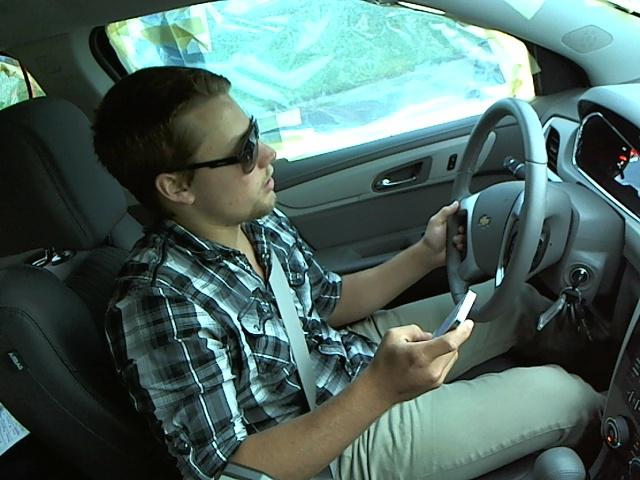
\includegraphics[width=0.9\textwidth]{img_6}
				\end{center}
			\end{column}
		\end{columns}
		
	\end{frame}
	
	\begin{frame}
		\frametitle{Task}
			\begin{center}
				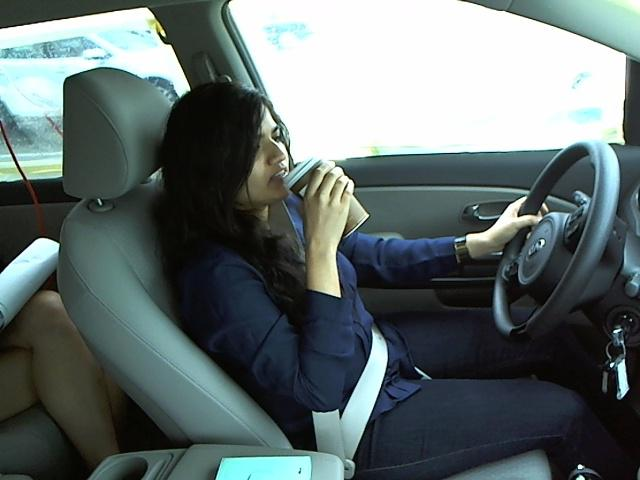
\includegraphics[width=5cm]{img_0} \vspace{0.1cm}
				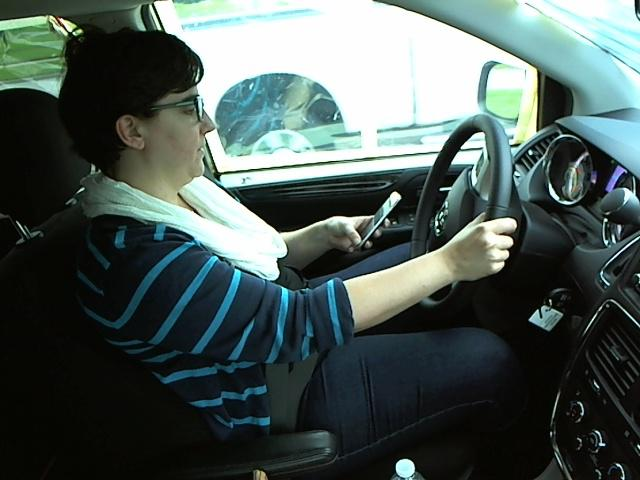
\includegraphics[width=5cm]{img_5} \\
				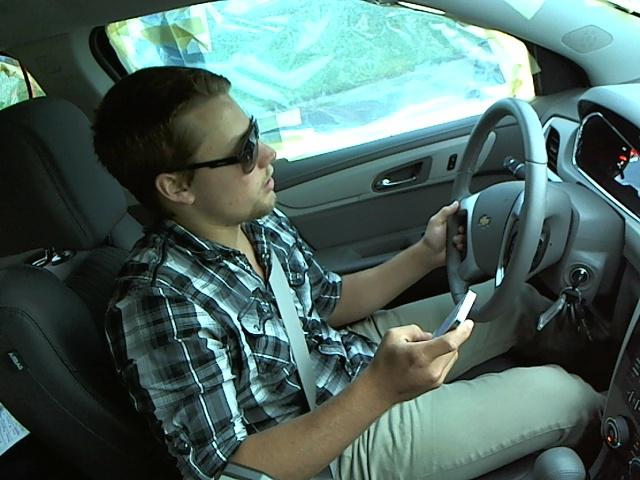
\includegraphics[width=5cm]{img_6}\vspace{0.1cm}
				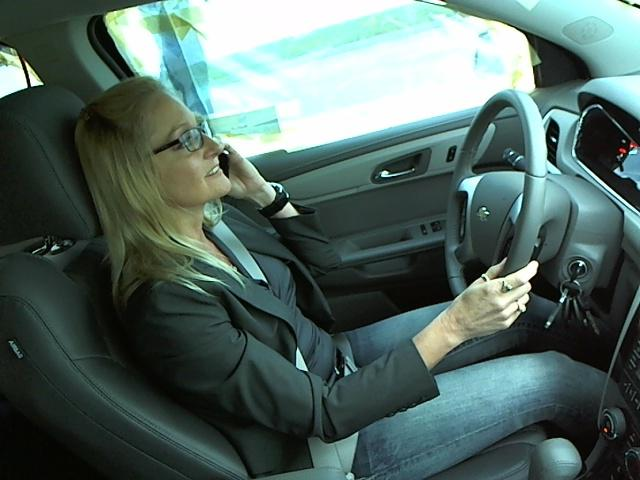
\includegraphics[width=5cm]{img_14}
			\end{center}
	\end{frame}
	
	\begin{frame}
		\frametitle{Task}
		\begin{center}
			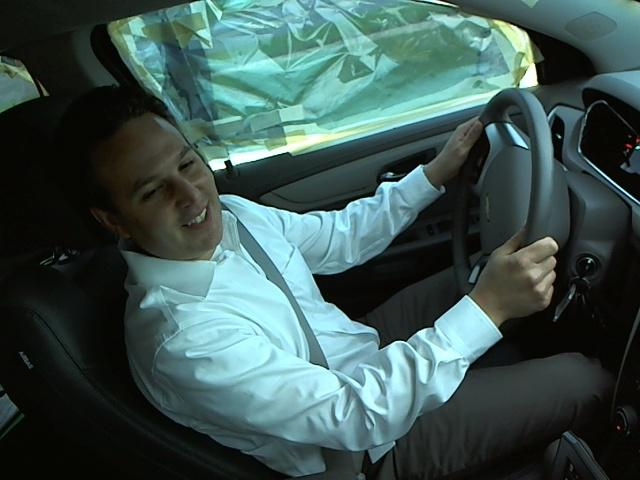
\includegraphics[width=5cm]{img_19} \vspace{0.1cm}
			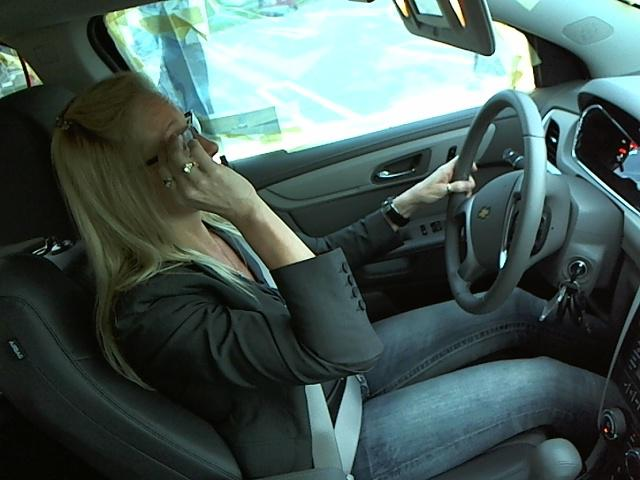
\includegraphics[width=5cm]{img_26} \\
			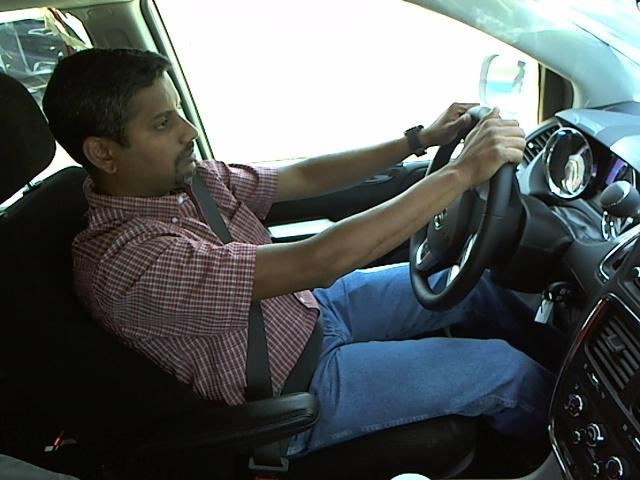
\includegraphics[width=5cm]{img_34}\vspace{0.1cm}
			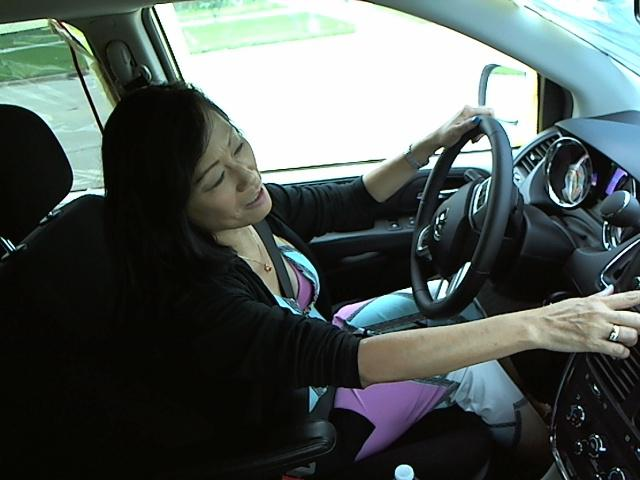
\includegraphics[width=5cm]{img_56}
		\end{center}
	\end{frame}
	
	\begin{frame}
		\frametitle{Task}
		\begin{center}
			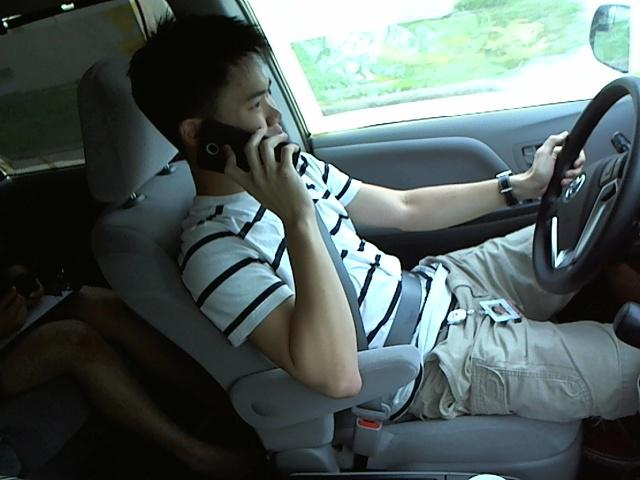
\includegraphics[width=5cm]{img_94} \vspace{0.1cm}
			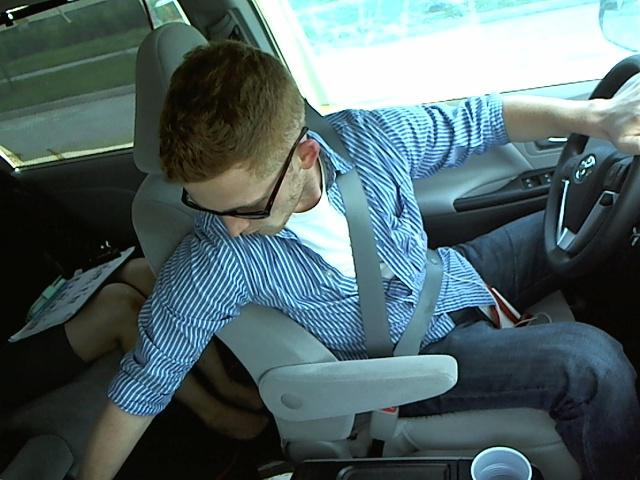
\includegraphics[width=5cm]{img_81} 
		\end{center}
	\end{frame}
	
	\begin{frame}
		\frametitle{Motivation}
		Distraction-affected crashes:
		\begin{itemize}
			\item 18\% of injury crashes
			\item 16\% of police-reported motor vehicle crashes
			\item 3000 people killed in the US per year
			\item 400,000 injured in the US per year
		\end{itemize}\\
		\vspace{0.2cm}
		Thus distraction-detection is important! \\
		\vspace{0.2cm}
		Using specialized sensors and trackers is too expensive! \\
		\vspace{0.2cm}
		Simple cameras combined with CV algorithms are non-intrusive and cheap!
	
	\end{frame}
	
	\begin{frame}
		\frametitle{Related Work}
		
		\begin{columns}
			\begin{column}{0.75\textwidth}
				Driver-Distraction Detection:
				\begin{itemize}
					\item Datasets mostly from cameras with frontal-views \cite{itsc:bergasa2008}
					\item Some approaches with specialized sensors (RGBD cameras etc.) \cite{Ragab2014}
					\item Often recorded in artificial environments
					\item Mostly rely on gaze-tracking or head-pose estimation
				\end{itemize}		
				Current methods are not applicable in our case!
			\end{column}
			\begin{column}{0.25\textwidth}  %%<--- here
				\begin{center}
					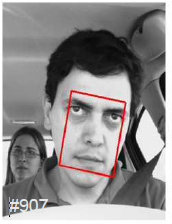
\includegraphics[width=0.9\textwidth]{frontal-view-dataset} \\
					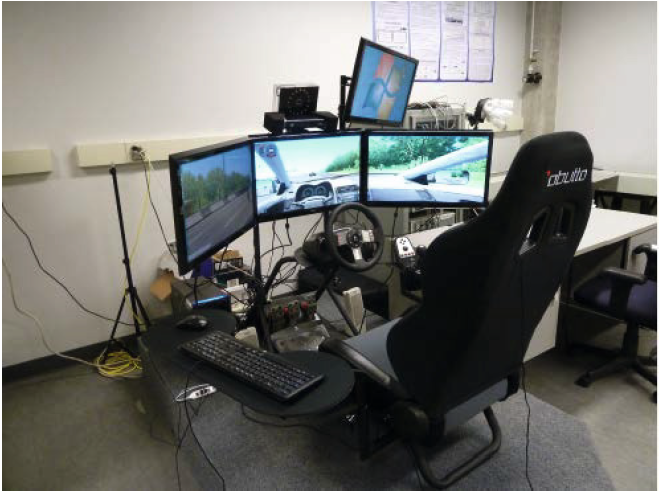
\includegraphics[width=0.9\textwidth]{RanForSim}
				\end{center}
			\end{column}
		\end{columns}
		
	\end{frame}
	
	\begin{frame}
		\frametitle{Related Work}
		
		\begin{columns}
			\begin{column}{0.75\textwidth}
				Activity Recognition:
				\begin{itemize}
					\item Often use different sensors (wearable sensors, smartphones)
					\item Camera based ones rely on continues video

				\end{itemize}		
				Current methods are not applicable in our case!
			\end{column}
			\begin{column}{0.25\textwidth}  %%<--- here
				\begin{center}
					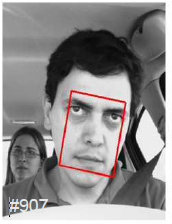
\includegraphics[width=0.9\textwidth]{frontal-view-dataset} \\
					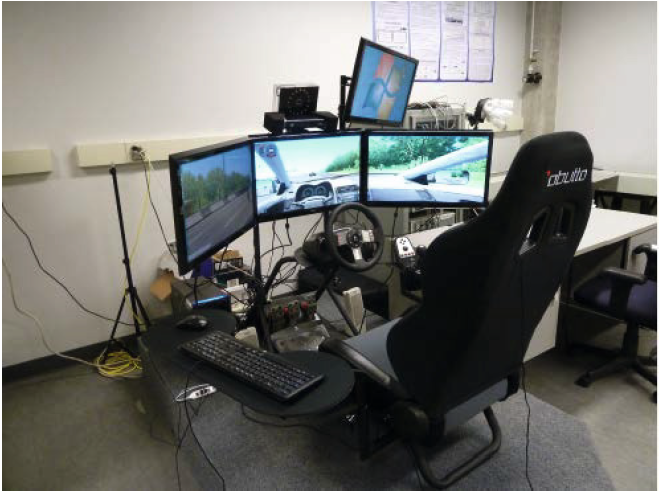
\includegraphics[width=0.9\textwidth]{RanForSim}
				\end{center}
			\end{column}
		\end{columns}
		
	\end{frame}
	
	
	\section{Models, Tools, Novelty}	

    \begin{frame}
        \frametitle{Tentative Material and Methods}
        Technologies we consider using:
        \begin{itemize}
            \item Support Vector Machines (based on SIFT and HOG features)
            \item Random Forests
            \item using Matlab
            \item AlexNet in Caffe
            \item Off-the-shelf head-pose estimator (for example FACE)
        \end{itemize}

    \end{frame}

    \begin{frame}
		\frametitle{Investigation}
        \begin{center}
	        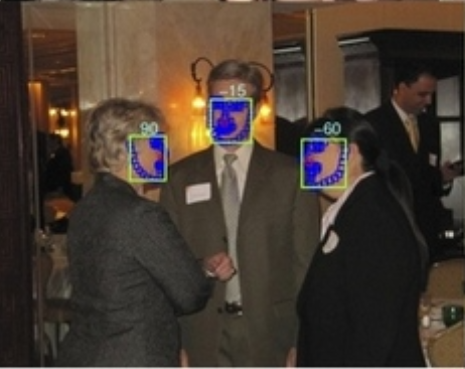
\includegraphics[width=0.4\textwidth]{head-pose} \\ \vspace{0.1cm}
	        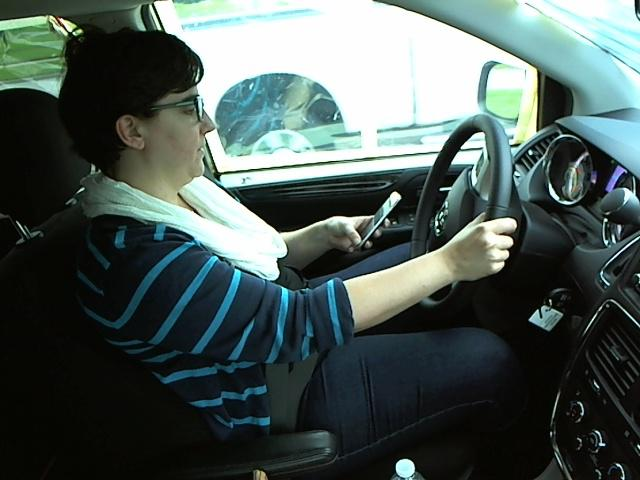
\includegraphics[width=0.35\textwidth]{img_5} \hspace{0.1cm}
	        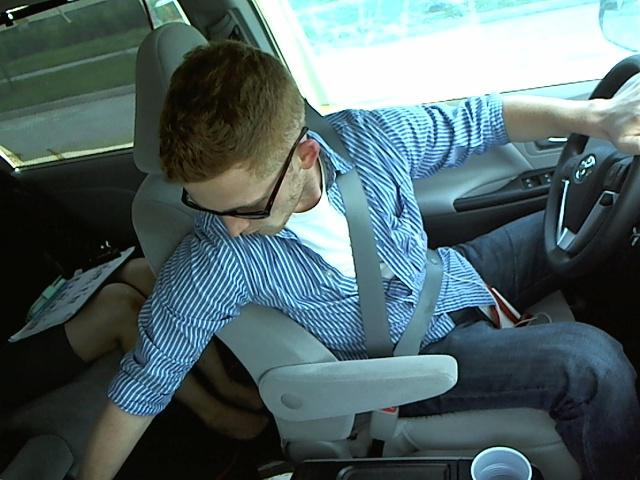
\includegraphics[width=0.35\textwidth]{img_81}
			\newline
			Head-pose could distinguish several of the classes clearly
        \end{center}
    \end{frame}

    \begin{frame}
		\frametitle{Investigation}
        \begin{center}
        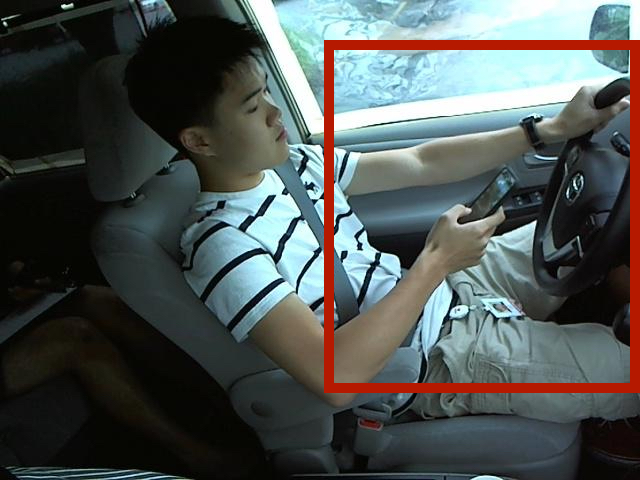
\includegraphics[width=9cm]{images/HandLocalisation.jpg}\\
        Rough classification in vicinity of the steering wheel using a hard-coded cropped version of our picture\end{center}
    \end{frame}


    \begin{frame}
		\frametitle{Investigation}
        \begin{center}
        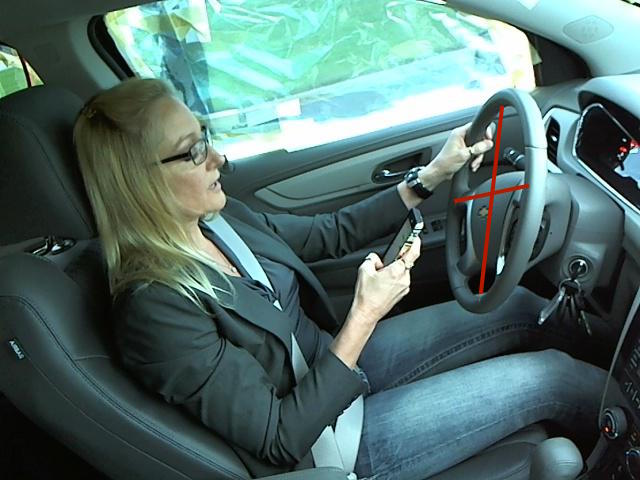
\includegraphics[width=9cm]{images/CameraPose.jpg}\\
        Camera-pose estimation using the steering-wheel pose\end{center}
    \end{frame}


    \begin{frame}
		\frametitle{Investigation}
        \begin{center}
        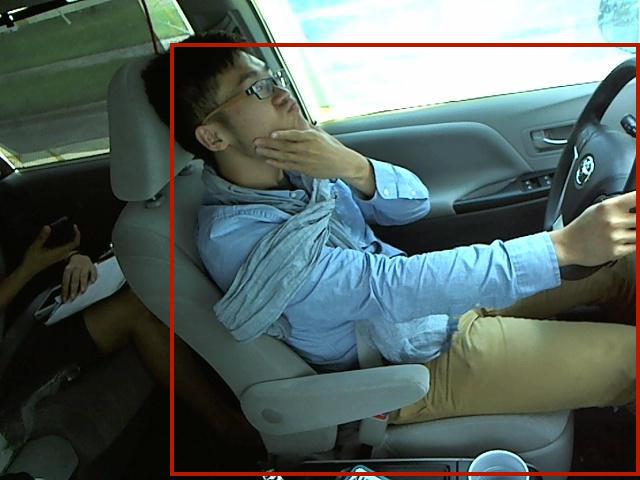
\includegraphics[width=9cm]{images/BoundingBox.jpg}\\
        Estimating Bounding-Box surrounding the driver to reduce search space potentially using the detected face and steering-wheel pose\end{center}
    \end{frame}

	
	\section{Analysis}	
	\begin{frame}
		\frametitle{Benchmark}
		\begin{itemize}
			\item 2,200 labeled images in training set provided by competition
			\item 80,000 unlabeled images in test set
			\item Test set consists of drivers not included in the training set
			\item Multi-class logarithmic loss: $$logloss = - \frac{1}{N} \sum_{i=1}^N \sum_{j=1}^M y_{ij} \log (p_{ij})$$
			
		\end{itemize}
		


	\end{frame}

		
		


		
		\begin{frame}[allowframebreaks]
			\frametitle{References} 
			\nocite{*} 
			\bibliographystyle{amsalpha} 
			\bibliography{references} 
		\end{frame}
		
		\medskip	
		

	
		

\end{document}
